\section{Optimization}
\begin{itemize}
    \item Describe circuit graphs
    \item Give formal definition
    \item Example graph
\end{itemize}

\subsection{Optimization Rules}
\begin{itemize}
    \item Described in Sec.~\ref{sec:background_circuitOptimization}
\end{itemize}

\subsection{Circuit Graph}
\label{sec:concept_circuitGraph}
\begin{itemize}
    % Quick link to paper: https://quantum-journal.org/papers/q-2023-11-08-1176/pdf/
    % \item Why rules could be applied directly to code, can be tedious and error prone, must adjust for many cases
    % \item eg 2 consecutive gate on one wire may be separated by many gate applications (on separate wires) in code
    % \item abstraction in useful
    % \item Rules applied to circuit graph described by \cite{KMO*23}
    % \item describe graph
    % \begin{itemize}
        % \item Graph acyclic and directed
        % \item Input and output node for each qubit
        % \item Each has only one outgoing or incoming vertex respectively
        % \item For each gate node with as many input and output vertices as qubit parameters (e.g. H gate 1 in and out and CX 2 in and out respectively)
        % \item Each vertices pair (of incoming and outgoing vertex) represent a node to which the gate is applied
        % \item Therefore, for each qubit, there exists one path from its input node to its output node such that all gates that are applied to it are visited in order of application
    % \end{itemize}
    \item Create graph from program code
    \begin{itemize}
        \item How to systematically create graph
        \item Get all declaration
        \item Foreach, create input/output node pair
        \item \dots
    \end{itemize}
    \item Apply optimization rules to graph instead of code
    \begin{itemize}
        \item (Systematically) iterate through subgraphs 
        \item Check if there is an equivalent, more efficient/cost-effective subgraph
        \item replace subgraph with optimized one 
    \end{itemize}
\end{itemize}
While it is possible to directly apply optimizations to the program code or internal representation of that code, this approach can be tedious and error prone. For example, the easiest approach would be to iterate over the code and search for code sequences with more efficient but equivalent alternatives, similar to the peephole optimization pattern on classical computers presented in Sec.~\ref{sec:background_codeOptimization}. However, two consecutive gates operating on a single wire may be separated by multiple gate applications on different wires in the programmatic description. Therefore, many simple optimization rules may not be applied when using a simplistic algorithm. A more complex approach would be too subdivide the program into lists of gate application where the wires being operated on by each list are disjunct. While this approach can result in the application of more optimization rules, it will also miss possible applications and already requires a complex implementation. Furthermore, improving on this method only increases its complexity and, in turn, makes it more prone to errors. Therefore, the language does not directly apply the optimizations to the program but uses a circuit graph description, based on the graph described by Kreppel et al.~\cite{KMO*23}, to apply the optimizations.

The circuit graph is a graphical description of a quantum graph; it is a acyclic and directed graph. For each qubit in the circuit, there exist both an input node and an output node. Furthermore, each input node as exactly one outgoing vertex while each output node as exactly one incoming vertex. Besides the input and output nodes, all other nodes represent gates in the circuit. All gate nodes the number of incoming vertices is equivalent to the number of outgoing vertices. Additionally, the number of incoming, or outgoing, vertices is the same as the number of parameters of the gate. Importantly, in this case, any qubits controlling the application of the gate, \eg the first qubit in a controlled-not gate, do also count to the number of parameters. In turn, their exists a vertices pair of an incoming and outgoing vertex each that represent a qubit to which the gate is applied. Therefore, for each qubit, there exists one path from its input node to its output node such that all gates that are applied to it are visited in order of application.

An example of a simple, unoptimized circuit graph is depicted in Fig.~\ref{fig:circuit_graph_unoptimized}. For simplicity, all applied gates are depicted in their corresponding node of the circuit graph. The circuit consist of three qubits, $q_0$, $q_1$, and $q_2$. Firstly, an $X$ is applied to the first qubit $q_0$. Than, a controlled-not gate is applied to the first two qubits $q_0$ and $q_1$, where $q_0$ is the controlling qubit. Similtaniously, two Hadarmard gates $H$ are applied to the thrid qubit $q_2$. Lastly, another $X$ gate is applied to the first qubit $q_0$ while another controlled-not gate is applied to the second and thrid qubits $q_1$ and $q_2$. In this case, the second qubit $q_1$ is the controlling qubit.
\begin{figure}[htp]
    \centering     
    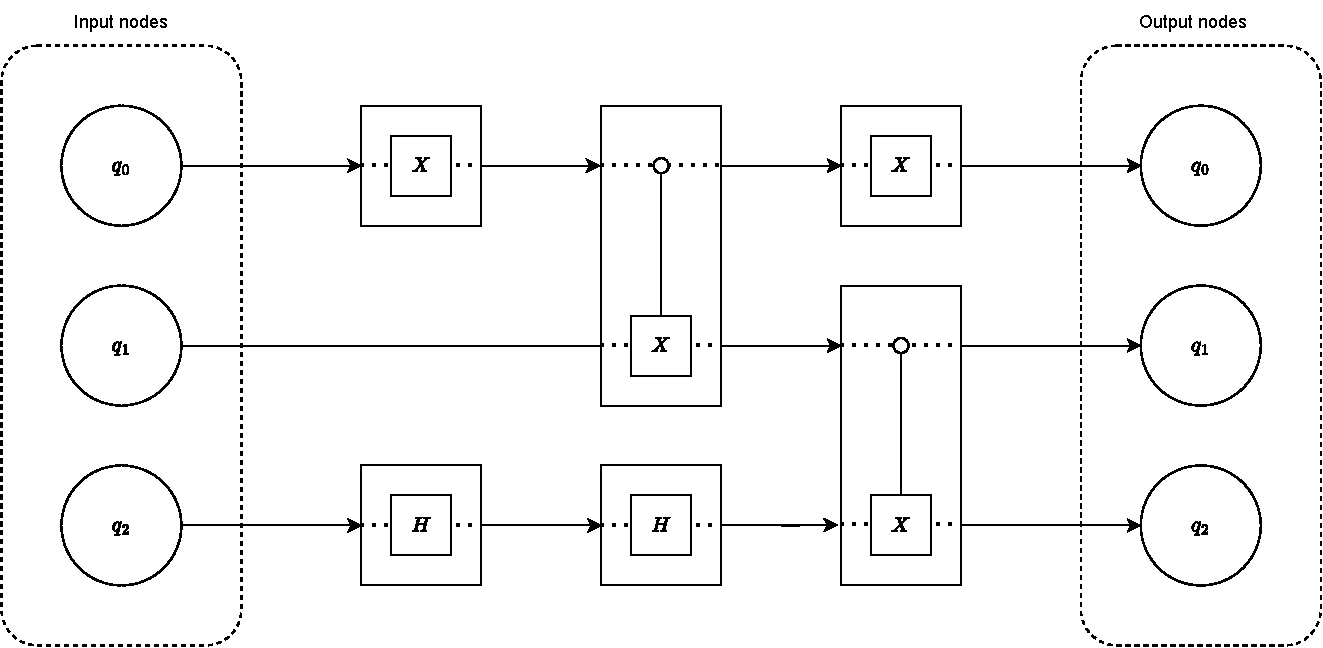
\includegraphics[width=.8\textwidth]{../figures/circuit_graph_unoptimized.pdf}
    \caption{An example of a simple, unoptimized circuit graph.}
    \label{fig:circuit_graph_unoptimized}
\end{figure}